\section{Combining and recasting limits}\label{sec:21.5}

Two silicon crystals cut from one wafer and read by identical sensors differ by more than two orders of magnitude in their event rate between 3 and \SI{38}{eV}, because one of them is glued to its holder (\cref{sec:19.6-lee}). The lowest pair bins of a charge detector carry a dark rate, charge that leaks across the gap without any deposit (\cref{sec:1.5-quanta}). No model predicts either rate to the accuracy that a background subtraction needs, so the Poisson limit with a known background of \cref{sec:21.4} cannot be applied to them as it stands. A limit is also rarely the last use of a measurement. A second experiment wants to add its exposure to the first, and a later calculation of the response, such as the background screening of a Dirac material (\cref{sec:16.1}), changes the expected signal after the limit has been published. We will set limits that hold for any background, combine searches in one likelihood whose theory nuisances are shared, and derive when a published limit can be recast to a new response without the data.

\subsection{Limits with an unknown background}\label{sec:21.5-unknown}

If part of the background may be unknown, the only expectation that can safely be assumed for it is zero. Counting every observed event as signal then gives the classical limit of \cref{sec:1.5}: the 90 percent upper limit $N_{\mathrm{sig}}^{\mathrm{lim}}$ solves $P(N \le N_{\mathrm{obs}}\,|\,N_{\mathrm{sig}}) = 0.10$ with the Poisson probabilities \cref{eq:1.5-poisson}, which gives 2.303, 3.890, 5.322 and 6.681 for zero to three events. The limit holds whatever the background is. The distribution function $P(N \le n\,|\,\mu)$ falls monotonically with the mean, since its derivative with respect to $\mu$ is $-P(N = n\,|\,\mu)$, so a signal that leaves a probability below 0.10 for so few events leaves even less once a background $N_{\mathrm{bkg}} \ge 0$ is added to it. The price is that every event, background or not, weakens the limit.

Using the shape of the expected signal gives a stronger limit. At fixed $\mchi$ the spectrum $\dd N_{\mathrm{sig}}/\dd E$ in the measured variable $E$ is known up to the factor $\sigmae$, and a background of a different shape crowds its events where the signal is small, typically near threshold. Yellin's maximum-gap method uses this~\cite{yellin2002finding}. Measure each position by the expected signal count below it, $x(E) = \int^E(\dd N_{\mathrm{sig}}/\dd E')\,\dd E'$. In this variable the signal events of any spectrum are spread uniformly with unit density over $[0, N_{\mathrm{sig}}]$, and the size of a gap between two adjacent events, or between an event and an end of the range, is the signal count expected inside it. For a signal-only experiment the probability that the largest gap is smaller than $x$ depends only on $x$ and $N_{\mathrm{sig}}$~\cite[Eq.~(2)]{yellin2002finding}:
\begin{equation}
  C_0(x, N_{\mathrm{sig}}) = \sum_{k=0}^{m}\Bigl[(kx - N_{\mathrm{sig}})^k - k\,(kx - N_{\mathrm{sig}})^{k-1}\Bigr]\frac{\ee^{-kx}}{k!} , \qquad m = \lfloor N_{\mathrm{sig}}/x\rfloor ,
  \label{eq:21.5-C0}
\end{equation}
written in the form that stays finite when $N_{\mathrm{sig}}/x$ is an integer; Yellin's printed form has the factor $1 + k/(N_{\mathrm{sig}} - kx)$ in place of the bracket, which is the same function away from those points. The 90 percent limit is the cross-section at which the observed largest gap has $C_0 = 0.90$. At fixed mass the fraction $g$ of the expected signal inside the largest gap does not depend on $\sigmae$, so $N_{\mathrm{sig}}^{\mathrm{lim}}$ solves $C_0(gN_{\mathrm{sig}}, N_{\mathrm{sig}}) = 0.90$. With no events the only gap is the whole range, $g = 1$. Then only $k = 0$ and $k = 1$ contribute, the $k = 1$ term is $-\ee^{-N_{\mathrm{sig}}}$, and $C_0 = 1 - \ee^{-N_{\mathrm{sig}}}$ recovers $N_{90} = 2.303$ of \cref{eq:1.5-N90}. The method stays valid with any background: added events can only split gaps, never widen them, so the observed largest gap is no larger than the signal alone would have left, and the limit errs on the conservative side.

How much the shape buys depends on where the events fall. One event that leaves 90 percent of the expected signal on one side gives $g = 0.90$ and $N_{\mathrm{sig}}^{\mathrm{lim}} = 2.836$, against 3.890 from counting. The same event in the middle of the signal, $g = 0.5$, gives 7.78, twice the counting limit; the two methods break even at $g = 0.761$. Two events that both lie in the lowest tenth of the expected signal, where a background rising toward threshold would put them, give $g = 0.90$ and again 2.836, against 5.322 from counting, while two events that cut the signal into thirds give 13.8. The maximum gap gains where the background sits apart from the signal and loses heavily where events are spread through it, and since the method is fixed before the data are seen, an experiment chooses it for the background it expects.

When the events are dense, a gap may be the wrong interval. The optimum-interval method generalizes it~\cite[Sect.~III]{yellin2002finding}. Let $C_n(x, N_{\mathrm{sig}})$ be the probability that, in a signal-only experiment, every interval containing at most $n$ events has an expected count no larger than $x$. It too depends only on $x$ and $N_{\mathrm{sig}}$; it is computed by Monte Carlo and equals \cref{eq:21.5-C0} for $n = 0$. We evaluate $C_n$ for the observed events on every interval bounded by events or by the ends of the range, $(N_{\mathrm{obs}} + 1)(N_{\mathrm{obs}} + 2)/2$ intervals, each with its own $n$ and $x$, and take the largest value, $C_{\mathrm{Max}}$. The 90 percent limit is the cross-section at which $C_{\mathrm{Max}}$ equals the value that 90 percent of signal-only experiments stay below, again from Monte Carlo. That calibration accounts for the interval having been chosen after the data were seen. Both methods need an ordered, continuous variable such as a phonon energy. Integer pair counts leave the events of one bin unordered, and for them the binned analog is a Poisson limit per bin, combined as in \cref{sec:21.5-recast}.

Neither method has a likelihood, since the unknown background has none, and so a theory nuisance cannot be profiled in it: \cref{eq:C.14-profile} needs $\mathsf{L}$. A normalization nuisance scales $N_{\mathrm{sig}}$ at fixed shape, and the band it puts on the limit is the envelope, $(1 + \delta_k)^{\pm1}$, of first order in $\delta_k$, where a likelihood would have charged the second-order cost of \cref{eq:21.4-profile}. A tilt also changes the fractions $g$, because the gaps are measured in expected counts, and the limit must be recomputed with the tilted spectrum at $\vartheta_k = \pm1$.

\subsection{Combining searches with shared nuisances}\label{sec:21.5-combine}

The counts of two exposures are independent, so their Poisson likelihoods multiply (\cref{eq:C.14-poisson}). A combination of experiments $X = \mathrm{A}, \mathrm{B}, \dots$ is one likelihood, the product of the single-exposure likelihoods \cref{eq:8.8-like},
\begin{equation}
  \mathsf{L}\bigl(\sigmae, \vartheta, \vartheta^{\mathrm{det}}\bigr) = \prod_X\mathsf{L}^{(X)}\bigl(\sigmae, \vartheta, \vartheta^{\mathrm{det},(X)}\bigr) .
  \label{eq:21.5-comb}
\end{equation}
Every theory nuisance $\vartheta_k$ appears once and acts in every factor, while the detector nuisances $\vartheta^{\mathrm{det},(X)}$, an efficiency, a background normalization or an energy calibration, are one set per experiment with constraints of their own (\cref{sec:21.4}). The theory nuisances are shared because a truncation is a property of the calculation (\cref{sec:8.8}), and every experiment that uses the same computed response inherits the same error. With one $\vartheta_k$ per experiment the profile could pull them in opposite directions and fit a difference between the experiments that no calculation can produce. It also pays the constraint once for each, as if the errors were independent, and so understates the cost of the truncation.

Before the product, the signal of every experiment is recomputed from one response at one truncation label, since published signal models from different codes differ by more than many of the truncations do. The tabulation spread of \cref{sec:21.4-like} enters \cref{eq:21.5-comb} as one more shared nuisance, not as an error of each experiment. Conventions that differ between publications, the local density, the halo parameters and the pair-creation model that turns energy into pair bins, are choices, not uncertainties, and they are removed by the recomputation, not profiled. Every search on Earth sees the same halo, so if its parameters are varied, one set of them acts on all factors, and near the edge they enter only through the combinations of \cref{sec:21.3-degeneracy}. And searches in different materials share the halo and the nuisance of each truncation that is computed the same way for both, with templates $\delta_k$ of their own and one $\vartheta_k$ (\cref{sec:8.8}). The limit is then set from \cref{eq:21.5-comb} as from a single likelihood (\cref{sec:21.4}).

\begin{workedexample}{Combining two silicon exposures}\label{we:21-combine}
Take $\mchi = \SI{10}{MeV}$, a heavy mediator, the standard halo of \cref{sec:1.2} and the one-pair bin of the cascade of \cref{sec:18.3}, the bin that sets the standard-halo limit at this mass in \cref{sec:21.2-iso}. The tabulated silicon response of \cref{sec:10.1} gives $r = \SI{9.14e41}{kg^{-1}.yr^{-1}.cm^{-2}}$ in this bin, that is 0.914 events per kg-year at $\sigmae = \SI{e-42}{cm^2}$. Exposure A has $M_{\mathrm{det}}t_{\mathrm{exp}} = \SI{1}{kg.yr}$, no events and no background. Exposure B has \SI{4}{kg.yr}, three events and a known background of 2.5 events. Both use the same response, which carries one normalization nuisance, $(1 + \delta)^{\vartheta}$ with $\delta = 0.25$, the size of the largest truncations of the silicon rate at \SI{10}{MeV} in \cref{tab:10-nuisances}.

\emph{Construction.} The limit is the Neyman construction of \cref{sec:21.4-like}. For each $\sigmae$ we sum the Poisson probabilities of all outcomes $(N_{\mathrm{A}}, N_{\mathrm{B}})$ up to 60 events each whose statistic \cref{eq:C.14-profile} is at least the observed one, with the nuisance at its conditional best fit $\hat{\hat\vartheta}$ to the observed counts and the constraint term held fixed. The 90 percent limit is the $\sigmae$ at which that probability is 0.10.

\emph{Without the nuisance.} Exposure A alone excludes $2.303/0.914 = \SI{2.52e-42}{cm^2}$, and B alone $\SI{1.14e-42}{cm^2}$; its three events above a background of 2.5 cost less than its fourfold exposure gains. Together they exclude $\SI{0.809e-42}{cm^2}$, 0.32 of A and 0.71 of B. At the combined limit A expects 0.74 signal events and B 2.96.

\emph{One shared nuisance.} With \cref{eq:21.5-comb} and one $\vartheta$ the limit is $\SI{0.897e-42}{cm^2}$, a factor 1.109 above the combination without it. The profile pulls the nuisance to $\hat{\hat\vartheta} = -0.46$, toward less signal, in both factors at once.

\emph{One nuisance per exposure.} Treated as two independent parameters, the nuisances settle at $-0.17$ (A) and $-0.29$ (B), and the limit is $\SI{0.851e-42}{cm^2}$, a factor 1.051. Splitting the nuisance halves its cost, and the limit is too strong by \SI{5}{\percent}. The worst case within one standard deviation, $\vartheta = -1$, would cost the full factor 1.25.

\emph{One exposure.} For A alone the shared construction gives a closed form. With no events only the outcome $N_{\mathrm{A}} = 0$ has a statistic as large as the observed one, so the limit is reached when the profiled expectation $u = N_{\mathrm{nom}}(1 + \delta)^{\hat{\hat\vartheta}}$ satisfies $\ee^{-u} = 0.10$, $u = N_{90}$. The profile condition of \cref{sec:8.8}, $\hat{\hat\vartheta} = -ku$ with $k = \ln(1 + \delta)$, then gives $N_{\mathrm{nom}} = N_{90}\,\ee^{k^2N_{90}}$, a cost of 1.12 for $\delta = 0.25$, which is \cref{eq:21.4-profile} with $\sigma_\beta = k$ and $\mathsf{t}' = 2N_{90}$.
\end{workedexample}

\subsection{Recasting a published limit}\label{sec:21.5-recast}

A published limit $\sigmae^{\mathrm{lim}}(\mchi)$ was computed with the rates $r_j^{\mathrm{pub}}(\mchi)$ per unit cross-section in the bins $j$ of its analysis. A later calculation replaces them by $r_j^{\mathrm{new}}(\mchi)$, and we write the ratio as the recast factor of bin $j$,
\begin{equation}
  K^{\mathrm{rc}}_j(\mchi) = \frac{r_j^{\mathrm{pub}}(\mchi)}{r_j^{\mathrm{new}}(\mchi)} .
  \label{eq:21.5-K}
\end{equation}
If $K^{\mathrm{rc}}_j = K^{\mathrm{rc}}$ in every bin, the correction preserves the shape of the expected signal at each mass. Every expected count is then $N_{\mathrm{sig},j} = \sigmae M_{\mathrm{det}}t_{\mathrm{exp}}r_j^{\mathrm{new}} = (\sigmae/K^{\mathrm{rc}})M_{\mathrm{det}}t_{\mathrm{exp}}r_j^{\mathrm{pub}}$. Any procedure that depends on $\sigmae$ only through the expected counts, which includes a Poisson limit per bin, a profile likelihood over many bins and Yellin's two methods, returns the limit $K^{\mathrm{rc}}\sigmae^{\mathrm{lim}}$. The recast is then exact without the data.

If $K^{\mathrm{rc}}_j$ varies from bin to bin, the correction tilts the expected spectrum, and the recast needs the procedure. One procedure can be recast exactly: a limit defined as the smallest of single-bin limits, $\sigmae^{\mathrm{lim}} = \min_jN_j^{\mathrm{up}}/(M_{\mathrm{det}}t_{\mathrm{exp}}r_j^{\mathrm{pub}})$, with the upper counts $N_j^{\mathrm{up}}$ of the bins published. Replacing $r_j^{\mathrm{pub}}$ by $r_j^{\mathrm{new}}$ in that minimum is the new limit. If only the curve is public, the new limit is still bracketed. Each new single-bin limit is $K^{\mathrm{rc}}_j$ times the old one, and every old one is at least $\sigmae^{\mathrm{lim}}$, so the new minimum is at least $(\min_jK^{\mathrm{rc}}_j)\,\sigmae^{\mathrm{lim}}$. The bin $j^*$ that set the published limit still offers $K^{\mathrm{rc}}_{j^*}\sigmae^{\mathrm{lim}}$, so the new minimum is at most that. A profile likelihood over several bins and the optimum interval have no such form. Their limits depend on how the counts are spread over bins or events and on all the $r_j$ together, and no function of the published curve and the $K^{\mathrm{rc}}_j$ reproduces them. Recasting them needs the binned likelihood, or the event list.

\begin{keyresult}[Recasting a limit to a new response]
With the recast factors \cref{eq:21.5-K}, a published limit $\sigmae^{\mathrm{lim}}(\mchi)$ becomes
\begin{equation}
  \sigmae^{\mathrm{lim,new}}(\mchi) =
  \begin{cases}
    K^{\mathrm{rc}}(\mchi)\,\sigmae^{\mathrm{lim}}(\mchi) & \begin{tabular}[t]{@{}l@{}}if $K^{\mathrm{rc}}_j = K^{\mathrm{rc}}$ for all $j$\\(any procedure),\end{tabular}\\[2pt]
    \min_j N_j^{\mathrm{up}}\big/\bigl(M_{\mathrm{det}}t_{\mathrm{exp}}\,r_j^{\mathrm{new}}(\mchi)\bigr) & \begin{tabular}[t]{@{}l@{}}if the limit is a minimum over bins\\with $N_j^{\mathrm{up}}$ public\end{tabular}
  \end{cases} ,
  \label{eq:21.5-recast}
\end{equation}
and both forms are exact. For a minimum over bins known only through its curve,
\begin{equation}
  \min_jK^{\mathrm{rc}}_j \le \frac{\sigmae^{\mathrm{lim,new}}}{\sigmae^{\mathrm{lim}}} \le K^{\mathrm{rc}}_{j^*} \le \max_jK^{\mathrm{rc}}_j ,
  \label{eq:21.5-bracket}
\end{equation}
with $j^*$ the bin that set the published limit. A correction that varies between bins cannot be recast from the curve of a profile-likelihood or optimum-interval limit.
\end{keyresult}

A minimum over bins carries a cost in confidence. If each of $n$ independent bins is set at 90 percent, the minimum excludes a true signal whenever any one bin does, and it covers with probability $0.9^n$: 0.81 for two bins and 0.73 for three. The union bound of \cref{sec:21.2-program} restores the stated level. A minimum over bins is recastable exactly only with this correction included in the published $N_j^{\mathrm{up}}$.

Halo conventions show both cases of \cref{eq:21.5-recast}. Take a silicon limit at \SI{10}{MeV} with the search of \cref{sec:21.2-iso}: one kg-year, empty one-, two- and three-pair bins of the cascade and $N_j^{\mathrm{up}} = \ln 30$. It was computed with the halo of Essig et al., $v_0 = 230$, $v_{\mathrm{esc}} = 600$, $v_{\mathrm{E}} = \SI{240}{km.s^{-1}}$ and $\rho_\chi = \SI{0.4}{GeV.cm^{-3}}$~\cite[App.~B]{essig2016direct}, and we recast it to the halo of \cref{app:A.8}. The density enters every rate as a factor, $K^{\mathrm{rc}} = 0.4/0.3 = 1.333$ in every bin, and recasts exactly with any procedure. The velocity distribution does not: at fixed density its recast factors are 0.953, 0.903 and 0.866 in the three bins. The old halo, with smaller $v_0$ and $v_{\mathrm{E}}$, has fewer fast particles in its bulk, and the higher bins need faster particles. With the density the factors are 1.271, 1.204 and 1.154. The published limit, \SI{2.93e-42}{cm^2}, was set by the one-pair bin, and the exact recast is \SI{3.72e-42}{cm^2}, a factor 1.271. From the curve alone, with the binding bin unknown, \cref{eq:21.5-bracket} gives 1.154 to 1.271. At \SI{2}{MeV} the factors are 1.156, 1.432 and 4.0 with the density (0.867, 1.074 and 3.0 without it). The higher bins now draw on the tail, which the old halo extends to $v_{\mathrm{max}} = \SI{840}{km.s^{-1}}$ against 794.5; the three-pair bin opens only above \SI{614}{km.s^{-1}}, and the binding one-pair bin gives 1.156.

The same rule decides how far a theory band can be recast. A normalization nuisance has one $\delta_k$ in every bin, and its band moves with the central limit. A tilt or a threshold shift has bin-dependent templates, and its band needs the per-bin limits or the likelihood, as the central value of any other tilted correction does. \Cref{tab:21-recast} sorts the corrections met in this book.

\begin{table}[tbp]
  \caption{Recast factors \cref{eq:21.5-K} of the corrections met in this book, and what a recast from a published curve needs. ``Common'' means the same factor in every bin at fixed $\mchi$, recastable exactly with any procedure. ``Bin-dependent'' means exact only for a single bin or for a minimum over bins with its upper counts public, and bracketed by \cref{eq:21.5-bracket} otherwise.}
  \label{tab:21-recast}
  \centering\small\setlength{\tabcolsep}{4pt}
  \begin{tabular}{@{}p{0.34\linewidth}p{0.20\linewidth}p{0.38\linewidth}@{}}
    \toprule
    Correction & Factor & Recast \\
    \midrule
    Local density $\rho_\chi$ & common & $\rho_\chi^{\mathrm{pub}}/\rho_\chi^{\mathrm{new}}$, exact \\
    Normalization nuisance (\cref{sec:8.8}) & common & $(1 + \delta_k)^{-\vartheta_k}$, exact, band included \\
    Background in the total $\varepsilon$, isotropic Dirac cone (\cref{sec:16.1}) & common & $\varepsilon_{\mathrm{bg}}^2$ for $\sigmae$, $\varepsilon_{\mathrm{bg}}^{1/2}$ for $\zeta$, exact \\
    Halo velocity distribution ($v_0$, $v_{\mathrm{esc}}$, $v_{\mathrm{E}}$) & bin-dependent & higher bins move most; at the edge through $E_{\mathrm{on}}/v_{\mathrm{max}}^2$ (\cref{sec:21.3}) \\
    Screening and local fields, tilt nuisances (\cref{sec:10.10}) & bin-dependent & templates per bin \\
    Gap or threshold shift & bin-dependent & moves the edge, \cref{we:21-gapshift} \\
    Anisotropic background tensor (\cref{sec:16.1-zrte5}) & depends on $\hat{\vect{q}}$ & ratio of event integrals per mass \\
    Relativistic density row of a boosted flux (\cref{sec:10.9}) & depends on speed & rate ratio $R$, limit $\times R^{-1/2}$ \\
    \bottomrule
  \end{tabular}
\end{table}

An exact recast of any procedure needs what its likelihood contains, and a publication that provides it can be reused without approximation: per bin the observed count, the expected background with its covariance, the exposure and efficiency, the response of the detector from deposited energy to bin with its nuisances, and the upper count with its confidence convention; the halo convention and the truncation label of the signal model; and the likelihood itself in machine-readable form.

\subsection{Dirac and boosted-flux recasts}\label{sec:21.5-corrected}

The published reaches of Dirac materials screen the dark-photon field by the Dirac electrons alone, and the total dielectric function adds the background $\varepsilon_{\mathrm{bg}}$ of the remote bands (\cref{sec:16.1}). For an isotropic cone the published loss function is $\varepsilon_{\mathrm{bg}}^2$ times the true one at every $(\vect{q}, \omega)$, and the published absorption rate $\varepsilon_{\mathrm{bg}}$ times the true one (\cref{eq:16.1-ratio}). The factor is common to every bin and every mass, so by \cref{eq:21.5-recast} the corrected reach is the published curve times $\varepsilon_{\mathrm{bg}}^2$ in $\sigmae$, and times $\varepsilon_{\mathrm{bg}}^{1/2}$ in the mixing $\zeta$, since the absorption rate grows as $\zeta^2$. Nothing else multiplies it: the published $|\varepsilon_{\mathrm{pub}}|^2$ already contains the renormalization of the Dirac charge, $|1 + \varepsilon_{\mathrm{D}}/\varepsilon_{\mathrm{bg}}|^{-2}$, with $\varepsilon_{\mathrm{D}}$ the polarization of the Dirac electrons (\cref{sec:16.1,app:D.41}). \Cref{fig:21-dirac-recast}a recasts the ideal material of Hochberg et al., with $\varepsilon_{\mathrm{bg}} = 40$~\cite{hochberg2018detection}. The minimum of its gapped curve, \SI{3.4e-46}{cm^2} near \SI{9}{keV}, becomes \SI{5.4e-43}{cm^2}, as in \cref{we:16-factor}, and at \SI{114}{keV} the gapless curve moves from \SI{5.5e-45}{cm^2} to \SI{8.8e-42}{cm^2}.

\begin{figure}[tbp]
  \centering
  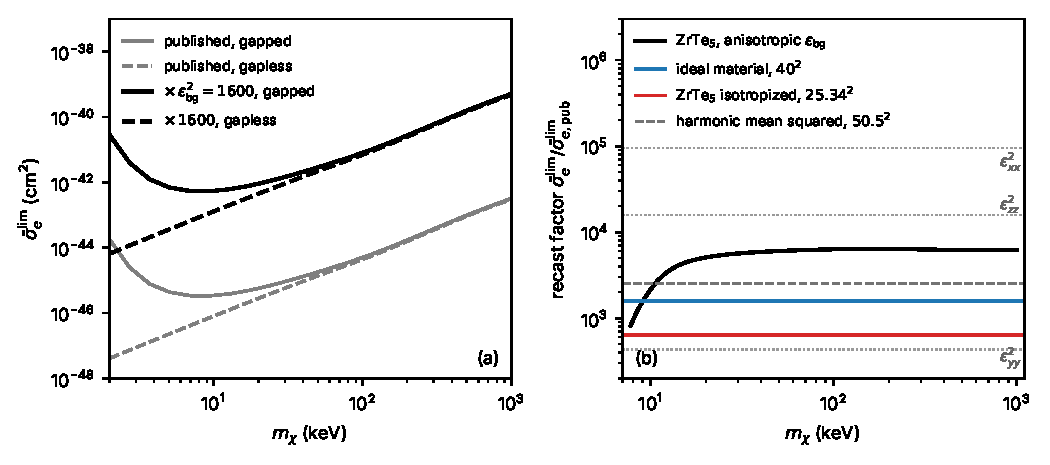
\includegraphics[width=\linewidth]{figures/ch21/fig21_5.pdf}
  \caption{Recasting published Dirac-material reaches to the total dielectric function; light mediator, three events in one kg-year, no background. (a) The ideal Dirac material of Hochberg et al.~\cite{hochberg2018detection} ($v_{\mathrm{D}} = 4\times10^{-4}$, $\varepsilon_{\mathrm{bg}} = 40$, $g_{\mathrm{deg}} = 2$, cutoff \SI{0.2}{keV}): published curves (gray), gapped ($\Delta_{\mathrm{D}} = \SI{2.5}{meV}$, solid) and gapless (dashed), read from the reference's figure. Black: the same curves times $\varepsilon_{\mathrm{bg}}^2 = 1600$, exact for any procedure because the factor is the same at every $(\vect{q},\omega)$. (b) Recast factor, the ratio of the corrected to the published reach, against $\mchi$. Black: the ratio of the published-rule to the total-$\varepsilon$ event integral at each mass for ZrTe$_5$ (\cref{sec:16.1-zrte5}). It uses the anisotropic background tensor $\varepsilon_{\mathrm{bg},ii} = 308.4$, 20.75, 126.1 and the measured-structure row of Geilhufe et al.~\cite{geilhufe2020dirac} ($\Delta_{\mathrm{D}} = \SI{11.8}{meV}$), the book's halo and the rate averaged over orientations of the crystal. Flat lines: $40^2 = 1600$ (blue) and $25.34^2 = 642$ for the isotropized ZrTe$_5$ of Hochberg et al. (red), both exact; the square of the harmonic mean of the tensor, $50.5^2 = 2554$ (gray dashed); the on-axis factors $\varepsilon_{\mathrm{bg},ii}^2 = 431$, $1.6\times10^4$ and $9.5\times10^4$ (gray dotted).}
  \label{fig:21-dirac-recast}
\end{figure}

An anisotropic crystal has no common factor. Its published rule divides each component of the Dirac polarization by its own $\varepsilon_{\mathrm{bg},ii}$, the total dielectric function adds the background along $\hat{\vect{q}}$, and their ratio depends on the direction of $\vect{q}$ and on $(q, \omega)$ (\cref{eq:D.41-ratio}). The published ZrTe$_5$ reach is, however, a single count, three events with no background, and a single bin is the case $n = 1$ of a minimum over bins: the recast is exact once both event integrals are computed at each mass. Their ratio is 5100 to 6400 between \SI{20}{keV} and \SI{1}{MeV} (\cref{fig:21-dirac-recast}b). Toward the threshold it falls, to 2200 at \SI{10}{keV} and 820 at \SI{7.7}{keV}, because only momentum transfers near the $y$ axis, with the lowest threshold, \SI{7.1}{keV}, and the smallest background constant, remain kinematically allowed there, and along that axis the factor is $\varepsilon_{\mathrm{bg},yy}^2 = 431$. No constant reproduces the curve: the square of the harmonic mean of the tensor, the natural isotropic guess, is low by a factor of two to two and a half above \SI{20}{keV} and high near threshold.

A boosted flux changes the counting itself. Dark matter accelerated by cosmic rays acquires its speed through the same coupling that the detector measures, so the flux is proportional to $\sigmae$ and the expected count to $\sigmae^2$, as the published analysis of silicon and germanium states~\cite{liang2025plasmon}. With $N^{\mathrm{up}}$ fixed, a change of the detection rate per particle by a ratio $R$ moves the lower edge of the excluded region by $R^{-1/2}$. For the exact density row of a relativistic particle, \cref{eq:10.9-Drel}, the ratios are those of \cref{sec:10.9-boosted}: the heavy-mediator limit is unchanged, the shift of $\sigmae$ for a massless mediator is below one percent for $\mchi \ge \SI{10}{keV}$, and below about \SI{3}{keV} it is undetermined. Settling it, with the transverse row and its Cherenkov pole included, is the recast that \cref{sec:10.9-open} leaves open and \cref{app:E.16} specifies.
